\documentclass[]{llncs}

\usepackage{graphicx}
% Used for displaying a sample figure. If possible, figure files should
% be included in EPS format.
%
% If you use the hyperref package, please uncomment the following line
% to display URLs in blue roman font according to Springer's eBook style:
% \renewcommand\UrlFont{\color{blue}\rmfamily}

% Display polish characters
\usepackage[utf8]{inputenc}
\usepackage{polski}
\usepackage{url}

% Translate some names to polish
\def\keywordname{{\bf Słowa Kluczowe:}}

\begin{document}

\title{Wykorzystanie Ethereum do Budowy Zdecentralizowanej Aplikacji}
\author{Wojciech Korzeniowski}
\institute{
  Instytut Informatyki\\Wydział Elektroniki i Technik Informacyjnych\\Politechnika Warszawska\\
  \url{http://www.ii.pw.edu.pl/}
}

\maketitle

\begin{abstract}

  Opis smart kontraktów zdefiniowanych na platformie Ethereum. Przykład
  wykorzystania Ethereum do zrealizowania zdecentralizowanego systemu do
  głosowania. Koniec artykułu zostanie poświęcony poszczególnym zagrożeniom
  wynikającym z wykorzystania smart kontraktów wraz z konsekwencjami ich
  przeoczenia

  \keywords{Ethereum \and Smart kontrakt \and Blockchain \and Decentralized Application \and DApp}

\end{abstract}

\section{Ethereum}

  Ethereum jest zdecentralizowaną platformą dla aplikacji które działają
  dokładnie tak jak zostały zdefiniowane bez możliwości oszustwa, cenzury czy
  interwencji stron trzecich\cite{ethereum}. Została stworzona przez rosyjskiego
  programistę nazywającego się Vitalik Buterin.

  Ether jest kryptowalutą wykorzystywaną na platformie Ethereum. Pod względem
  wartości rynkowej jest drugą co do wielkości kryptowalutą na świecie, zaraz po
  Bitcoinie\footnote{Według serwisu \url{https://coinmarketcap.com/}, stan na
  2.06.2018}.

  To co wyróżnia Ethereum na tle Bitcoina to fakt iż pozwala on na definiowanie
  smart kontraktów. To z kolei umożliwia tworzenie nowego rodzaju aplikacji
  nazywanych DApp, czyli Decentralized Application, co w wolnym tłumaczeniu z
  języka angielskiego oznacza "zdecentralizowana aplikacja". Są to aplikacje
  które wykorzystują smart kontrakty, lub bardziej ogólnie blockchain, jako
  miejsce do przechowywania danych aplikacji.

\section{Smart kontrakt}

  Smart kontrakt jest kolejnym etapem rozwoju technologii blockchain. Można
  znaleźć tłumaczenia które opisują smart kontrakt jako cyfrowy zapis umowy
  która w odpowiednich warunkach realizuje ustaloną akcję. Z technicznego punktu
  widzenia jest to zbiór danych oraz funkcji które mogą operować na danych i są
  jedynym sposobem na ich zmianę. Wywołania niektórych funkcji wymagają
  przekazania Etheru który może być przechowywany w smart kontrakcie jak w
  zwykłym portfelu lub być przekazanym dalej wraz z wywołaniem innej funkcji. Ma
  to miejsce na przykład w grach hazardowych gdzie aby wywołać funkcję losu
  należy przekazać ustaloną kwotę Etheru jako opłatę za los. W Ethereum smark
  kontrakty definiuje się wykorzystując język Solidity\cite{solidity}

  Istotną cechą która wynika z architektury blockchainu jest fakt iż smart
  kontrakt który został utworzony na blockchainie nie może zostać zmieniony.
  Jest to bardzo istotne ze względu na bezpieczeństwo tworzonej aplikacji.
  Jeżeli popełnimy błąd w definicji kontraktu nie ma możliwości jego naprawy.
  Jedyne co można zrobić to utworzyć nowy kontakt i zaprzestać korzystania z
  jego starej wersji. Takie rozwiązanie nie zawsze jest satysfakcjonujące,
  szczególnie jeżeli do starej wersji kontraktu przypisany jest Ether a nie
  utworzyliśmy funkcji która pozwala na jego przekazanie do innego portfela. Z
  drugiej strony istnienie funkcji która pozwala na wybranie całego Etheru z
  kontraktu może wzbudzić podejrzenia co do intencji jego twórcy.

\subsection{System do głosowania}

  Smart kontrakty mogą zostać wykorzystane do zbudowania systemu do tajnego
  głosowania. Organizator głosowania tworzy umowę z osobami uprawnionymi do
  głosowania która pozwala uprawnionym na oddanie dokładnie jednego głosu.
  Następnie, po zamknięciu głosowania, opcja która zebrała najwięcej głosów
  zostaje zwycięzcą głosowania.

  Zastanówmy się najpierw jakie są problemy w organizowaniu głosowania bez smart
  kontraktów. Przede wszystkim należy zadbać o to aby głos mogła oddać tylko
  osoba do tego upoważniona oraz aby każda z tych osób mogła oddać tylko jeden
  głos. Kolejnym problemem jest sposób w jaki głosy są liczone. Jak powiedział
  Józef Stalin: "Nieważne, kto głosuje, ważne, kto liczy głosy."

  Powyższe problemy w przypadku głosowań w Polsce rozwiązywane są przez
  Państwową Komisję Wyborczą która organizuje i pilnuje porządku głosowania.
  Tworzone są okręgowe komisje wyborcze których odpowiedzialnością jest
  kontrolowanie czy osoba oddająca głos jest do tego uprawiona. Następnie
  komisja skrutacyjna liczy głosy po czym ogłaszany jest wynik głosowania.

  Takie rozwiązanie wymaga istnienia tak zwanej "zaufanej trzeciej strony". W
  przypadku wyborów w Polsce jest to PKW. Obywatele muszą zaufać że komisja w
  poprawny sposób zorganizuje i przeprowadzi głosowanie a następnie bezbłędni
  policzy głosy i ogłosi zwycięzcę.  Nie raz pojawiały się różnego rodzaju
  kontrowersje co do sposobu przeprowadzania wyborów. Na przykład podczas
  wyborów samorządowych 2014 opóźnione było ogłoszenie wyników.  PKW tłumaczyła
  to awarią systemów informacyjnych jednak co bardziej podejrzliwi obywatele
  wyczuwali w tym spisek. Dodatkowo obywatele muszą ufać że każda z okręgowych
  komisji wyborczych będzie przestrzegać prawa i nie nadużyje swoich kompetencji
  aby sfałszować organizowane wybory.

  W przypadku głosowania zrealizowanego na smart kontraktach nie ma potrzeby
  istnienia zaufanej trzeciej strony. Można zdefiniować kontrakt którego
  definicja jest publicznie dostępna i każdy może sprawdzić w jaki sposób
  zbierane są głosy oraz jak są one zliczane. Wymaganie aby każdy z uprawionych
  mógł zagłosować tylko jeden raz można zrealizować poprzez przekazanie każdemu
  uprawnionemu jednego tokenu do głosowania który nie może być przekazany dalej.
  Osoba która wykorzystuje swój token do zagłosowania wywołuje odpowiednią
  funkcję na kontrakcie do głosowania w efekcie czego liczba głosów na wybraną
  opcję zwiększa się.

  Jedną z głównych zalet realizacji systemu głosowania opartego na blockchainie
  jest jego transparentność. Ponieważ dane zapisane na blockchainie są
  publicznie dostępne do odczytu każdy z zainteresowany może sprawdzić jak
  przebiegało głosowanie oraz jaki jest jego aktualny stan. Ponadto technologia
  blockchain gwarantuje że dane zapisane w blockchainie nie zostaną zmienione
  więc nie ma możliwości fałszowania wyników.

\section{Token}

  Tokenem w świecie Ethereum nazywamy nową "kryptowalutę" która istnieje na
  blockchainie Ethereum. Istnieje przyjęty interfejs tokenu o nazwie `ERC20`
  który definiuje token o określonej liczbie gdzie każdy z tokenów jest
  równoważmy innemu.

  Tokeny mogą być wykorzystane do zbiórki pieniędzy co jest nazywane ICO
  (Initial Coin Offering) i jest odpowiednikiem określenia IOP (Initial Public
  Offering) znanego giełd papierów wartościowych. Przypuśćmy że właściciel
  startupu potrzebuje dofinansowania do swojego biznesu. Może on utworzyć token
  o dowolnej nazwie i totalnej liczbie tokenów. Następnie sprzedawać je za
  Ether. W ten sposób twórca pozyskuje Ether którym może płacić lub wymienić na
  inną walutę. W zależności od przyjętej polityki ICO, Kupujący token otrzymuje
  udziały w startupie lub możliwość wykorzystania tokenu w zamian za usługę
  realizowaną przez biznes twórcy tokenu.

  Za przykład może posłużyć serwis aukcyjny w którym za wystawienie produktu
  należy zapłacić tokenem. Ci którzy kupili token podczas ICO zorganizowanego
  przed uruchomieniem serwisu, mogą go teraz wykorzystać lub sprzedać go innym
  którzy chcą wystawić przedmiot na tym serwisie.

\section{Komunikacja z siecią Ethereum}

  Sieć Ethereum\cite{ethereum-doc} składa się z węzłów które komunikują się ze sobą aby ustalić
  wspólną wersję blockchainu. Węzeł to serwer który posiada lokalną kopię
  blockchainu od początku jego istnienia wraz ze wszystkimi transakcjami i smart
  kontraktami które zostały na nim zapisane. Dodatkowo węzeł implementuje
  protokół JSON-RPC poprzez który następuje komunikacja klienta z węzłem.
  Jednym z bardziej znanych klientów jest klient napisany w języku JavaScript o
  nazwie Web3.js\footnote{https://github.com/ethereum/web3.js/}. Wykorzystując
  go można stworzyć aplikację działającą w przeglądarce która komunikuje się
  bezpośrednio z węzłem Ethereum.

  Inną możliwością jest stworzenie własnego serwera który komunikuje sie z
  węzłem. Następnie aplikacja przeglądarkowa komunikuje się tylko z naszym
  serwerem bez bezpośredniej komunikacji z węzłem. Takie rozwiązanie może być
  wykorzystane w celu przyspieszenia aplikacji aby nie odpytywać węzeł o dane za
  każdym razem tylko przechowywać je w pamięci podręcznej na serwerze.

  Funkcje zdefiniowane w smart kontrakcie można podzielić na 2 kategorie. Te
  które czytają dane i te które je zmieniają. Jako że dostęp do danych z
  blockchainu jest publiczny i można stworzyć własny węzeł który jest pełną
  kopią blockchainu, dane można odczytać w każdej chwili. Inaczej jest w
  przypadku funkcji która modyfikuje stan kontraktu. Wynika to z faktu iż każdy
  z węzłów musi wywołać tę funkcję aby potwierdzić czy inne węzły również ją
  wykonały i stan blockchainu się zgadza. Operacja ta nazywana jest ustaleniem
  konsensusu pomiędzy węzłami. Fakt iż musimy wykonać tę funkcję na wszystkich
  węzłach powoduje że za jej wywołanie, wołający musi zapłacić. Walutą w
  której dokonuje się opłaty jest Gas który jest kupowany podczas zlecania
  wywołania funkcji.

  Ilość Gasu potrzebnego do wywołania funkcji jest proporcjonalna do złożoności
  obliczeniowej funkcji. Cena Gasu zależy od aktualnego obciążenia sieci oraz od
  tego czy chcemy aby nasza funkcja została wywołana jak najszybciej.

  Wywołania funkcji, utworzenie smart kontraktu oraz transfer Etheru na inne
  konto nazywamy transakcją. Wszystkie transakcje trafiają do puli transakcji
  (ang.  Transaction Pool). Transakcje z puli są akceptowane zaczynając od tych
  za które jest największa opłata ponieważ te są najbardziej korzystne dla
  kopaczy odpowiedzialnych za utrzymanie konsensusu.

\subsection{Utworzenie nowego smart kontraktu}

  Aby utworzyć nowy kontrakt należy utworzyć transakcję wraz z 
  Do tej pory opisałem w jaki sposób komunikować się z istniejącym kontraktem
  jednak w jaki sposób utworzyć nowy kontrat

\section{Bezpieczeństwo}

  Dane aplikacji są najczęściej centralnym punktem stworzonej aplikacji. Utrata
  danych może spowodować że aplikacja staje się mniej wygodna w
  użytkowaniu\cite{teatr-wspolczesny-utrata-danych} lub sprawa że użytkownicy
  tracą zaufanie stracić zaufanie do aplikacji\cite{nazwa-pl-utrata-danych}.

  Innym z problemów jest wyciek danych\cite{wyciek-danych-studentow}. W mojej
  opinii jest to gorszy scenariusz niż usunięcie danych ponieważ użytkownicy
  aplikacji (w przykładach z cytowanego artykułu - studenci) są narażeni na
  Jeżeli natomiast nastąpi wyciek danych zaufanie do twórców aplikacji maleje co
  może spowodować odpływ użytkowników.

  Ciężko ocenić który ze scenariuszy jest gorszy. Usunięcie danych może
  sparaliżować pracę użytkownika aplikacji lub nawet nieść konsekwencje prawne w
  przypadku utraty wrażliwych danych które są nie do odzyskania np. Dokumentacji
  podatkowych\cite{utrata-dokumentacji}. W przypadku utraty danych możemy
  przewidzieć jakie konsekwencje się z tym wiążą. Inaczej jest gdy nastąpi
  wyciek danych. Wyciek niesie niebezpieczeństwa które ciężko jest przewidzieć.
  Zdarzają się sytuacje w których serwis, świadomie lub nie, udostępnia czyjeś
  dane osobowe. W takim przypadku ciężko jest przewidzieć w jaki sposób takie
  dane zostaną użyte. Jedną z takich wpadek zaliczyło Poznańskie Centrum
  Superkomputerowo-Sieciowe które pozwalało na pobranie imienia, nazwiska oraz
  adresu zamieszkana po podaniu numeru PESEL\cite{dane-dzieci}. W niepowołanych
  rękach danie dane mogą stwarzać realne niebezpieczeństwo dla dzieci które
  ogranicza tylko wyobraźnia atakującego.

  Wykorzystanie technologii blockchain pozwala ograniczyć wymienione powyżej
  zagrożenia ponieważ usunięcie danych z blockchainu jest niemożliwe. Ciężko
  też mówić o wycieku danych ponieważ dane zapisane na blockchainie są
  publicznie dostępne. Oczywiście jeżeli chcemy przechowywać dane wrażliwe na
  blockchainie muszą one być zaszyfrowane i możliwe do odczytu tylko dla
  odpowiednich osób. Jeżeli szyfrowanie zostanie zrealizowane błędnie lub sam
  klucz szyfrujący zostanie przejęty przez atakującego możemy mówić o wycieku
  danych.

  Dodatkowo jak wspomniałem w rozdziale TODO, DApp może wykorzystywać tradycyjne
  bazy danych takie jak relacyjne czy NoSQL. W takim przypadku twórcy aplikacji
  muszą brać pod uwagę zarówno niebezpieczeństwa związane z wykorzystaniem
  wybranej bazy danych jak i te wynikające z użycia blockchainu które omówię w
  kolejnych podrozdziałach.

  TODO
  \cite{open-zeppelin}

\subsection{Generowanie liczb pseudolosowych}

\cite{liczby-losowe}

\section{Podsumowanie}

  Podsumowując, system do głosowania wykorzystujący blockchain nie wymaga
  istnienia zaufanej trzeciej strony co jest główną ideą przyświecającą smart
  kontraktom. Dzięki spisaniu zasad umowy w sposób jednoznaczny w interpretacji
  oraz gwarancji wykonania danych akcji po spełnieniu wcześniej przyjętych
  warunków możemy zawrzeć umowę z kimś komu nie musimy ufać bez potrzeby
  pośrednika w postaci notariusza.


\subsubsection{Third Section}
\paragraph{Fourth Level}
Lorem ipsum dolor sit amet, consectetur adipiscing elit.


%
% ---- Bibliography ----
%
% BibTeX users should specify bibliography style 'splncs04'.
% References will then be sorted and formatted in the correct style.
%
% \bibliographystyle{splncs04}
% \bibliography{mybibliography}
%
\begin{thebibliography}{splncs04}
  \bibitem{ethereum} Ethereum Homepage,
  \url{https://www.ethereum.org/}

  \bibitem{ethereum-doc} Ethereum Homestead
  \url{http://www.ethdocs.org/en/latest/}


  \bibitem{solidity} Solidity - dokumentacj
  \url{https://solidity.readthedocs.io/en/v0.4.24/}

  \bibitem{nazwa-pl-utrata-danych} Awaria w Nazwa.pl – klienci stracili dane, także z backupów,
  \url{https://niebezpiecznik.pl/post/awaria-w-nazwa-pl-klienci-stracili-dane-takze-z-backupow/}

  \bibitem{teatr-wspolczesny-utrata-danych} Teatr Współczesny zhackowany? Niestety to nie happening
  \url{https://niebezpiecznik.pl/post/awaria-w-nazwa-pl-klienci-stracili-dane-takze-z-backupow/}

  \bibitem{wyciek-danych-studentow} Wyszukiwarki studentów, publiczna lista usterek i niebezpieczne punkty ksero, czyli uczelnianych wpadek cz. IV
  \url{https://niebezpiecznik.pl/post/wyszukiwarki-studentow-publiczna-lista-usterek-i-niebezpieczne-punkty-ksero-czyli-uczelnianych-wpadek-cz-iv/}

  \bibitem{utrata-dokumentacji} Skutki utraty dokumentacji podatkowej
  \url{http://www.ordynacjapodatkowa.pl/artykul,1679,5273,skutki-utraty-dokumentacji-podatkowej.html}

  \bibitem{dane-dzieci} Jak pozyskać dane osobowe i adresy dzieci z twojej okolicy?
  \url{https://niebezpiecznik.pl/post/jak-pozyskac-dane-osobowe-i-adresy-dzieci-z-twojej-okolicy/}

  \bibitem{liczby-losowe} Predicting Random Numbers in Ethereum Smart Contracts
  \url{https://blog.positive.com/predicting-random-numbers-in-ethereum-smart-contracts-e5358c6b8620}

  \bibitem{open-zeppelin} OpenZeppelin
  \url{https://github.com/OpenZeppelin/zeppelin-solidity}

\end{thebibliography}


% ########## START OF SAMPLES

\newpage
\newpage

\section{Takie tam przydatne przykłady}
\begin{definition} text \end{definition}
\begin{case} text \end{case}
\begin{proof} text \end{proof}

\noindent Widać na równaniu:
\begin{equation}
  x + y = z
\end{equation}

Please try to avoid rasterized images for line-art diagrams and
schemas. Whenever possible, use vector graphics instead (see
Fig.~\ref{fig1}).

\begin{figure}
  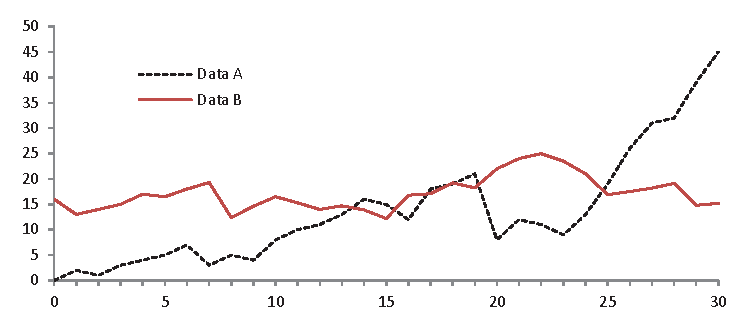
\includegraphics[width=\textwidth]{fig1.eps}
  \caption{A figure caption is always placed below the illustration.
    Please note that short captions are centered, while long ones are
  justified by the macro package automatically.} \label{fig1}
\end{figure}

Tabla~\ref{tab1} przedstawia że działa.

\begin{table}
  \caption{Table captions should be placed above the
  tables.}\label{tab1}
  \begin{tabular}{|l|l|l|}
    \hline
    Heading level &  Example & Font size and style\\
    \hline
    Title (centered) &  {\Large\bfseries Lecture Notes} & 14 point, bold\\
    1st-level heading &  {\large\bfseries 1 Introduction} & 12 point, bold\\
    2nd-level heading & {\bfseries 2.1 Printing Area} & 10 point, bold\\
    3rd-level heading & {\bfseries Run-in Heading in Bold.} Text follows & 10 point, bold\\
    4th-level heading & {\itshape Lowest Level Heading.} Text follows & 10 point, italic\\
    \hline
  \end{tabular}
\end{table}

% ########## END OF SAMPLES

\end{document}
